%Encoding: utf8
%Author: Pavol Loffay, xloffa00@stud.fit.vutbr.cz %Date: 16.10.2012
%Project: Dokumentácia k projektu MTU do predmetu ISA,

%preambule
\documentclass[12pt,a4paper,titlepage]{article}
\usepackage[slovak]{babel}
\usepackage[top=3.0cm, left=2.0cm, text={17cm, 24cm}]{geometry} 
\usepackage[IL2]{fontenc}
\usepackage[utf8]{inputenc}
\usepackage{verbatim}
\usepackage{graphics}
%\usepackage{hyperref}
\usepackage{times}
\usepackage[noline,ruled,longend,czech,algo2e]{algorithm2e} 
\newcommand\czuv[1]{\quotedblbase #1\textquotedblleft}

\begin{document}
\begin{titlepage}
    \begin{center}
    {\Huge \textsc{Vysoké učení technické v~Brně\\}} 
    {\huge \textsc{Fakulta informačních technologií\\}} 
    \bigskip
    \bigskip
    \bigskip
    \begin{center}
    \scalebox{0.3}{
\includegraphics{img/fit_logo.eps}} \end{center}
    \bigskip
    \bigskip
    \bigskip
    {\LARGE Dokumentácia k~projektu do predmetu ISA\\} 
    {\Huge Detekcia maximálneho MTU po ceste\\}
    \vspace{\stretch{0.618}}
    \end{center}

    \Large{\today \hfill Pavol Loffay}
    \bigskip
\end{titlepage}

\pagenumbering{roman}
\setcounter{page}{1}
\tableofcontents

\newpage
\pagenumbering{arabic}
\setcounter{page}{1}

\section{Úvod} \label{uvod}
    Tento dokument postupne popisuje teóriu, návrh riešenia a~implementáciu
    zisťovania maximálnej prenosovej jednotky, ďalej
    \emph{PMTU}\footnote{Path maximum transmission unit} z~jedného hostiteľa na druhého.
    Navrhnutý program pracuje ako konzolová aplikácia pre systém Linux.

    Dokument sa skladá z~viacerých časti. V~kapitole \ref{analyza} 
    sa venuje analýze problému a~popisuje techniky, ako sa dá
    zistiť maximálne \emph{PMTU}.Kapitola \ref{navrh} sa zoberá návrhom algoritmov.
    Ďalej nasleduje kapitola \ref{riesenie}, kde popisujeme ovládanie
    programu a~vlastnú implementáciu.

\section{Analýza problému a~princíp jeho riešenia} \label{analyza} 
    \subsection{Popis zadania}
    Úlohou tohto projektu bolo implementovať zistenie maximálnej
    prenosovej jednotky na ceste\,--\,\emph{PMTU}. V~prípade použitia \emph{IPv4}
    sme museli použiť bit zákaz fragmentácie, 
    skrátene\,--\,\emph{DF}\footnote{Don't fragment}. Pre implementáciu
    \emph{IPv6} neboli bližšie špecifikácie. Pre oba protokoly bolo
    určené použitie protokolov \emph{ICMP}\footnote{Internet Control
    Message Protocol} pre \emph{IPv4} a~analogicky \emph{ICMPv6}\footnote{Internet
    Control Message Protocol Version 6} pre \emph{IPv6}.

    Program mal pracovať ako konzolová aplikácia,
    pre operačne systémy založené na Unixu. Bolo špecifikovane 
    že máme použiť BSD schránky a~knižnice z~\texttt{netinet/*}
    a~pre preklad doménového mena \texttt{resolv.h} a~\texttt{netdb.h}.

    \subsection{MTU}
        Zisťovanie maximálnej prenosovej jednotky je veľmi dôležite.
        Pretože, ak by zdroj vysielal pakety ktoré sú väčšie ako 
        \emph{PMTU}, bude ich musieť niektorý zo sieťových uzlov fragmentovať.
        Tým pádom spracovanie jedného paketu bude náročnejšie a~bude trvať dlhšiu dobu.
        Naproti tomu ak by zdroj vysielal príliš male pakety, taktiež by dochádzalo
k~plytvaniu sieťových prostriedkov. Ešte musíme zmieniť, že pri
        fragmentácii, alebo vysielaní príliš malých paketov je väčšia pravdepodobnosť, že sa 
        pakety stratia pretože je ich väčšie množstvo.
        Preto je dôležité vhodne zvoliť čím najväčšiu prenosovú jednotku.

        \begin{figure}[htb!]
            \begin{center}
                \scalebox{1}{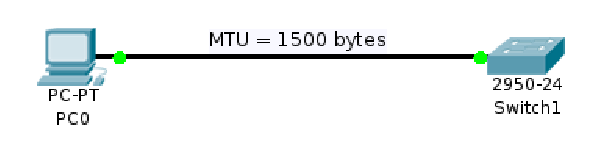
\includegraphics{img/mtu.eps}}
                \caption{\emph{MTU}\,--\,maximálna veľkosť prenosovej jednotky na jednom fragmente siete.}
                \label{mtu}
            \end{center}
       \end{figure}

        \begin{figure}[htb!]
            \begin{center}
                \scalebox{0.8}{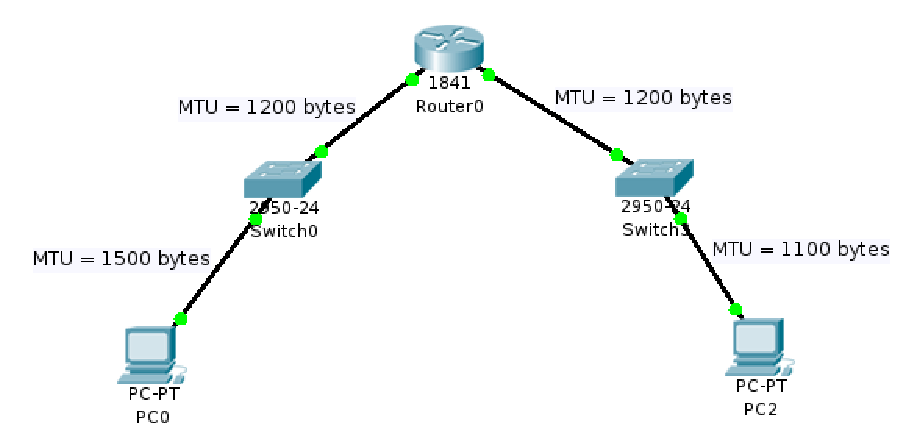
\includegraphics{img/pmtu.eps}} 
                \caption{\emph{PMTU}\,--\,maximálna veľkosť prenosovej jednotky na celej ceste.} 
                \label{pmtu}
            \end{center}
        \end{figure}

    \subsubsection{Ujasnenie pojmov MTU a~PMTU} 
        \emph{MTU\footnote{Maximum transmission unit}} charakterizuje maximálnu veľkosť prenosovej jednotky medzi
        dvoma zariadeniami, napríklad medzi počítacom a~rozbočovačom.
        \emph{PMTU}\,--\,maximálna veľkosť
        prenosovej jednotky medzi zdrojom a~cieľom po celej ceste. Čiže paket prejde
        viacerými segmentmi siete bez fragmentácie. \emph{PMTU} je znázornený na obrázku
        \ref{pmtu} medzi počítačmi \emph{PC0} a~\emph{PC2}, jeho veľkosť je \emph{1100 bajtov}.

    \subsection{PMTU pre IPv4}
        Protokol \emph{IPv4} je postavený tak, že smerovače
        ak je veľkosť paketu väčšia ako \emph{MTU} na odchádzajúcej linke,
        paket fragmentujú. Tým pádom musí byť tomu prispôsobenia aj hlavička
        \emph{IPv4}, kde je potom určené či je paket fragmentový a~následne poradie fragmentov.

        Pre zistenie maximálneho \emph{MTU} pre \emph{IPv4} je nutné použiť protokol \emph{ICMP}
a~korektne nastaviť hlavičku \emph{IPv4}, konkrétne bit zákazu fragmentácie\,--\,\emph{DF}
        bit viz \cite{rfc_pmtu}.
        Protokol \emph{IPv4} používa na zisťovanie stavu zariadení v~sieti protokol \emph{ICMP}.
        Ten je veľmi dôležitý a~typicky sa používa napríklad v~aplikáciach
        \texttt{ping} a~\texttt{traceroute}.
    
        Naša aplikácia bude posielať \emph{ICMP} správy \emph{Echo Request} s~rôznou veľkostnou, 
        pričom v~hlavičke IP paketu, musí byť nastavený bit zákaz fragmentácie. Následne bude 
        program čakať na prijatie \emph{ICMP} správy. Ak príde \emph{Echo Reply} znamená to, 
        že odoslaný paket bol korektne prijatý vzdialenou stanicou a~môžeme poslať väčší paket.
        Ak prijme správu \emph{ICMP Destination Unreachable} s~kódom 
        \emph{4}\footnote{fragmentation need and DF set}, znamená to že náš odoslaný paket 
        sa nedostal k~cieľovému zariadeniu pretože bola jeho velkosť väčšia ako niektoré
        \emph{MTU}, takže musíme zmenšiť objem posielaných dat.
        Týmto spôsobom veľmi jednoducho zistíme \emph{PMTU}.

    \subsubsection{Protokol ICMPv4}
        Tento protokol patri medzi najželezitejšie protokoly internetu. 
        Využívajú ho operačne systémy sieťových uzlov na posielanie rôznych 
        informačných a~chybových správ viz \cite{rfc_icmp}. Napríklad o~vypršaní
        \emph{TTL} alebo nedostupnosti služby. V~\emph{OSI} modele 
        ho môžme zaradiť k~Sieťovej vrstve. \emph{ICMP} správa je priamo obsiahnutá
        v~IP datagrame. V~tabuľke \ref{tabulka_icmp} môžeme vidieť, vybrané
        správy tohto protokolu.

        \begin{table}[h!]
            \begin{center}
                \begin{tabular}{llll}
                    $ \textbf{Nazov} $ & $ \textbf{Cislo typu} $ \\ $  Echo\ Reply $ & $ 0 $ \\
                    $  Destination\ Unreachable $ & $ 3 $ \\
                    $  Redirect $ & $ 5 $\\
                    $  Echo\ Request $ & $ 8 $\\
                    $  Time\ Exceed $ & $ 11 $\\
                    $  Parameter\ Problem $ & $ 12 $\\
                \end{tabular}
                \caption{Tabuľka vybranych \emph{ICMP} sprav.} \label{tabulka_icmp}
            \end{center}
        \end{table}

        Bližšie sa zameriame na popis \emph{ICMP} správy typu \emph{Echo Reply}
        a~\emph{Echo Request}. Tieto sa používajú na zistenie či je cieľový počítač dosiahnuteľný.
        Tento proces funguje následovne: zdrojový počítač pošle správu \emph{Echo Request}, ak túto
        správu obdrží zariadenie s~cieľovou adresou, tak odošle \emph{Echo Reply}. Tým pádom pôvodne
        zdrojové zariadenie zistí, že cieľová stanica je dostupná.

    \paragraph{Štruktúra správ Echo Request a~Echo Reply}
    \begin{figure}[h!]
        \begin{center}
            \scalebox{0.4}{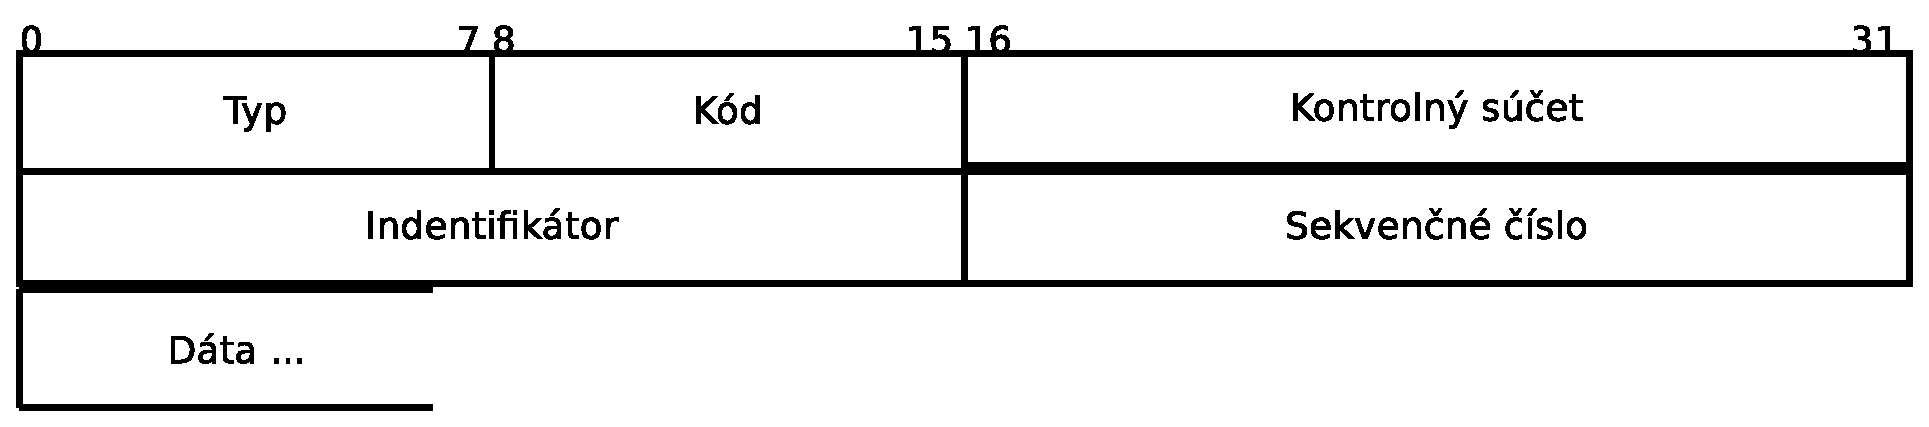
\includegraphics{img/echo1.eps}} 
            \caption{Struktura \emph{ICMP} správy \emph{Echo Request} a~\emph{Echo Reply}}
            \label{icmp_echo}
        \end{center}
    \end{figure}

    \begin{itemize}
        \item Typ: \emph{Echo Request 8} a~\emph{0} pre \emph{Echo Reply}.
        \item Kód: hodnota 0.
        \item Kontrolný súčet: \emph{16} bitový jednotkový doplnok súčtu jednotkového 
            doplnku celej \emph{ICMP} správy.
        \item Identifikátor: Nastavuje ho odosielateľ, prijímajúci uzol vytvorí odpoveď 
            s~identifikátorom odpovedajúcim k~prijatej správe. Podľa toho prijímateľ 
            rozlíši odpovede k~rôznym odoslaným správam.
        \item Sekvenčne číslo: každá vytvorená správa s~rovnakým identifikátorom musí
            mať iné sekvenčné číslo. Uzol ktorý odoslal \emph{Echo Request}, spozná odpoveď 
            ak sa bude zhodovať identifikátor a~sekvenčné číslo správy.
    \end{itemize}

    \paragraph{Štruktúra Destination Unreachable}
    \begin{figure}[h!]
        \begin{center}
            \scalebox{0.4}{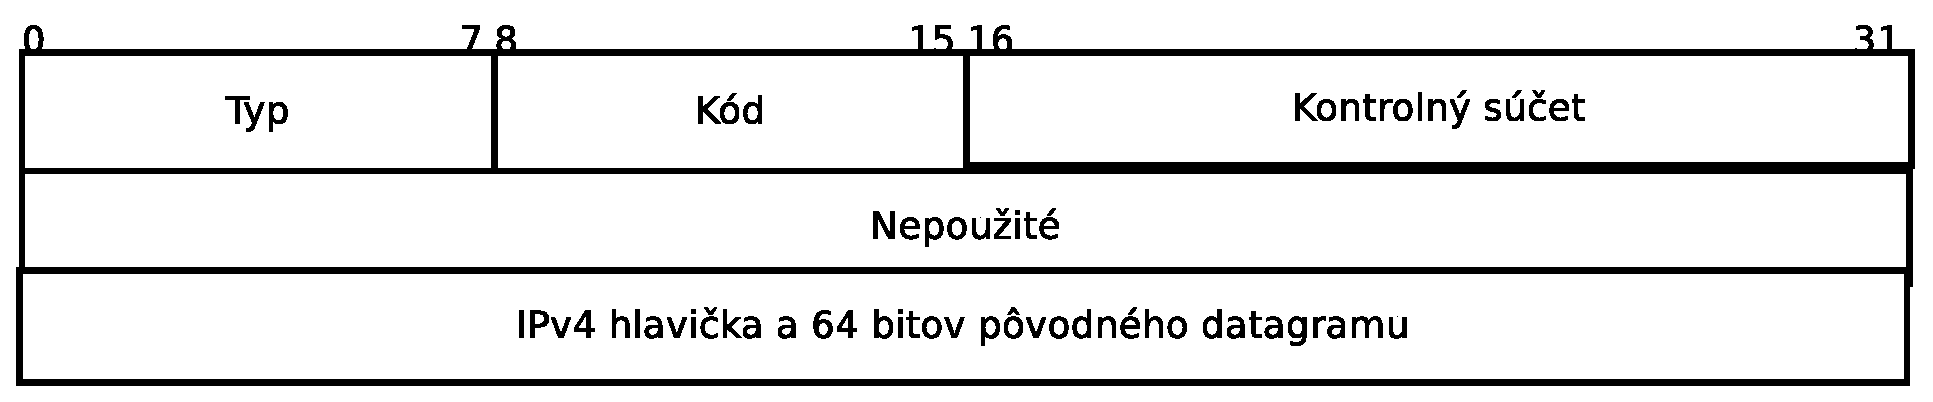
\includegraphics{img/icmp_destination_unreachable.eps}} 
            \caption{Struktura \emph{ICMP} správy \emph{Destination Unreachable}} 
            \label{icmp_des_unreachable}
        \end{center}
     \end{figure}
    
    \begin{itemize}
        \item Túto správu s~kódom \emph{4} používajú smerovače na oznamovanie že \emph{MTU}
            odchádzajúcej linky je menšie ako veľkosť paketu, avšak iba 
            tých ktoré majú nastavený \emph{DF} bit.
        \item Typ: nastavená hodnota na \emph{3}
        \item Kód: obsahuje hodnotu \emph{4}.
        \item Posledná položka: obsahuje pôvodne odoslanú \emph{IPv4} hlavičku
a~\emph{64} bitov pôvodného datagramu, čiže nami odoslanú \emph{ICMP} správu.
            Podla jej položiek identifikátor a~sekvenčne číslo zistíme
            či prijatá správa prislúcha k~nami odoslanej.
    \end{itemize}

    \subsection{PMTU pre IPv6}
        V~prípade použitia \emph{IPv6} musia koncové stanice zaistiť správnu
        veľkosť odosielaného paketu pretože na ceste nedochádza k~jeho fragmentovaniu.
        Aby sme mohli zistiť \emph{PMTU} pre \emph{IPv6} stačí použiť protokol
        \emph{ICMPv6}. Na rozdiel od \emph{IPv4} nemusíme upravovať hlavičku \emph{IPv6} 
        paketu, aby nedochádzalo k~fragmentácii.

        Na zistenie \emph{PMTU} pre \emph{IPv6}, budeme postupovať analogickým spôsobom
        ako pri \emph{IPv4}. Aplikácia bude posielať \emph{ICMPv6 Echo Request} správy s~rôznou veľkosťou.
        Ak prijmeme \emph{Echo Reply} prislúchajúcu k~nami odoslanému \emph{Echo Request} je
        zrejmé, že môžme zväčšiť veľkosť odosielaného paketu, pretože \emph{PMTU} 
        je menšie ako náš odoslaný paket.
        Ak niektoré \emph{MTU} po ceste je menšie ako odoslaná správa, sieťový uzol vygeneruje 
        \emph{ICMPv6} správu \emph{Packet Too Big} v~ktorej je veľkosť \emph{MTU} linky
        kde mal byť paket poslaný ďalej viz \cite{rfc_pmtuv6}.

    \subsubsection{Protokol ICMPv6}
        Jeho účel a~použitie je zhodný s~protokolom \emph{ICMPv4} avšak sa 
        používa pre \emph{IPv6}. Principálne obsahuje tie iste správy, ale kvôli
        miernym odlišnostiam \emph{IPv4} od \emph{IPv6} definuje nové správy, aby
        bola zaručená funkčnosť \emph{IPv6} viz \cite{rfc_icmpv6}.
    
        Tabuľka \ref{tabulka_icmpv6} ukazuje vybrané typy správ, môžme si všimnúť že 
        rovnaké správy pre \emph{ICMPv4} a~verziu \emph{6} majú iné hodnoty typu.

        Štruktúra správ \emph{ICMPv6} je pomerne zhodná s~\emph{ICMPv4}. Napríklad
        \emph{Echo Requst} a~\emph{Echo Reply} majú zhodnú štruktúru.

        \begin{table}[h!]
            \begin{center}
                \begin{tabular}{llll}
                    $ \textbf{Nazov} $ & $ \textbf{Číslo typu} $ \\ $  Echo\ Reply $ & $ 129 $ \\
                    $  Destination\ Unreachable $ & $ 1 $ \\
                    $  Redirect $ & $ 137 $\\
                    $  Echo\ Request $ & $ 128 $\\
                    $  Time\ Exceed $ & $ 3 $\\
                    $  Parameter\ Problem $ & $ 4 $\\
                    $  Packet\ Too\ Big $ & $ 2 $\\
                \end{tabular}
                \caption{Tabuľka vybraných \emph{ICMPv6} správ.} \label{tabulka_icmpv6}
            \end{center}
        \end{table}

        \begin{figure}[h!]
            \begin{center}
                \scalebox{0.4}{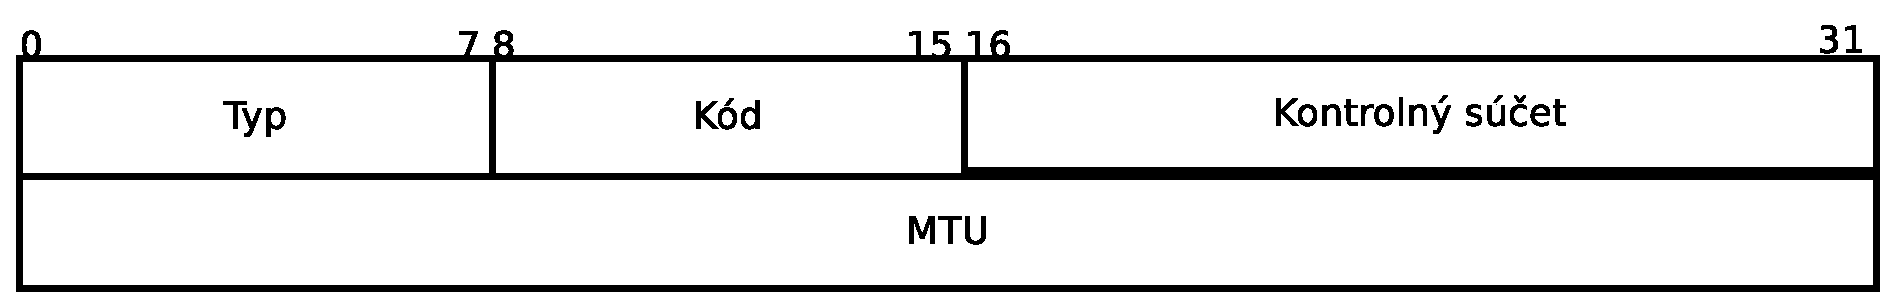
\includegraphics{img/icmpv6_packet_too_big.eps}} 
                \caption{Štruktúra \emph{ICMPv6} správy \emph{Packet Too Big}} 
                \label{icmp_packet_too_big}
            \end{center}
        \end{figure}

    \paragraph{Popis správy Packet Too Big}
        \begin{itemize}
            \item Tato správa je generovaná smerovačom na odpoveď paketu, ktorý
                nemôže 
                byť poslaný pretože je jeho veľkosť vačšia ako \emph{MTU} na
                odchádzajúcej linke.
            \item MTU: veľkosť \emph{MTU} na odchádzajúcej linke v~bajtoch.
        \end{itemize}

    \subsection{Problémy pri PMTU}
        Zisťovanie maximálnej prenosovej jednotky po celej ceste môže byť obtiažna 
        úloha, pretože nie všetky sieťové zariadenia vysielajú korektné \emph{ICMP} správy,
        alebo ich nevysielajú vôbec. Môže to byť spôsobené zlou konfiguráciou, alebo chybou 
        operačného systému smerovača. Bežnou chybou môže byť, že smerovače neposielajú 
        \emph{Destination Unreachable} s~kódom \emph{4}, čo znamená že na odchádzajúcom 
        rozhraní je menšie \emph{MTU} ako veľkosť paketu. Naša aplikácia by sa stým mala
        vyrovnať, tak že ak nepríde odpoveď do určitého času, zníži veľkosť paketu. 
        Niekedy taktiež môže dochádzať k~filtrovaniu paketov pomocou firewallu viz \cite{rfc_pmtu_problem}.

     \subsection{Binárne vyhľadávanie}
        Pre voľbu veľkosti posielaného \emph{ICMP Echo Request} paketu sme
        zvolili binárne vyhľadávanie, alebo inakšie nazývanú metódu rozpoľovania intervalu.
        Je to vyhľadávací algoritmus na nájdenie zadanej hodnoty v~usporiadanom zozname viz \cite{matematika_3}. 
        V~každom kroku skráti zoznam o~polovicu.
        Na základe výsledku porovnania sa rozhodne v~hornej alebo dolnej časti zoznamu 
        a~rekurzívne pokračuje od začiatku.

    \section{Návrh riešenia problému} \label{navrh}
        Po analýze problému, kde sme vysvetlili základne princípy a~teóriu ohľadne
        zisťovania maximálnej prenosovej jednotky, nasleduje abstraktný popis algoritmov.
        Taktiež tu ukážeme voľbu hodnôt veľkosti paketu.

    \subsection{Minimálna veľkosť paketu pre IPv4} 
        Každý internetový prvok musí byť schopný poslať datagram o~veľkosti \emph{68}
        bajtov bez ďalšej fragmentácie viz \cite{rfc_ip}.

    \subsection{Popis algoritmu pre IPv4} \label{algoritmus_ipv4} 
        Predpokladajme tri premenné \emph{minimálna}, \emph{maximálna} a~\emph{aktuálna} veľkosť paketu.

    \begin{enumerate}
        \item Nastav \emph{minimálnu} veľkosť \emph{MTU} na \emph{68} bajtov.
        \item Nastav \emph{maximálnu} hodnotu na \emph{1500} bajtov, alebo
            podľa zadaného parametru \texttt{-m <mtu>}.
        \item Nastav \emph{aktuálnu} dĺžku paketu \texttt{(minimálna veľkosť + maximálna veľkosť) / 2}.
        \item Vytvor \emph{IPv4} hlavičku s~nastaveným \emph{DF} bitom. K~hlavičke
            pripoj \emph{ICMP Echo Reguest} správu. Celková veľkosť musí byť rovná \emph{aktuálnej} veľkosti.
        \item Pošli vytvorený paket a~zapni časovač.
        \item Ak sa nepodarilo poslanie nastav \emph{maximálnu} veľkosť na \emph{aktuálnu}
            a~choď na bod 3.
        \item Prijímaj pakety pokiaľ nepríde \emph{Echo Reply},
            alebo \emph{Destination Unreachable} s~kódom \emph{4}. Oba odpovedajúce na náš paket.
        \item Ak prišiel \emph{Echo Reply} nastav \emph{minimálnu} veľkosť na \emph{aktuálnu}
            veľkosť a~choď na bod 3.
        \item Ak prišiel \emph{Destination Unreachable} s~kódom \emph{4}, 
            nastav \emph{maximálnu} veľkosť na \emph{aktuálnu} a~choď na bod 3.
        \item Ak vypršal časovač a~neprišiel \emph{ICMP} paket, tak nastav \emph{aktuálnu}
            veľkosť na \emph{maximálnu} veľkosť a~choď na bod 3.
        \item Opakuj body 3 až 10 pokiaľ nie je \emph{maximálna} veľkosť zhodná
                    s~\emph{minimálnou}.
        \item \emph{Aktuálna} veľkosť paketu udáva veľkosť \emph{PMTU}.
    \end{enumerate}

    \subsection{Minimálna veľkosť paketu pre IPv6} 
        Podla \cite{rfc_ipv6} musí každý sieťový prvok s~\emph{IPv6} protokolom pripojený
        na linku s~\emph{MTU 1280} bajtov. Avšak pre experimentálne účely sme zvolili minimálnu 
        veľkosť na \emph{150} bajtov.

    \subsection{Popis algoritmu pre IPv6} \label{algoritmus_ipv6} 
        Predpokladajme premenné \emph{minimálna}, \emph{maximálna} a~\emph{aktuálnu} veľkosť,
        ďalej premennú indikujúcu, že bola prijatá \emph{ICMP Packet Too Big} správa s~názvom \emph{too\_big}.

    \begin{enumerate}
        \item Nastav \emph{minimálnu} veľkosť \emph{MTU} na \emph{150} bajtov.
        \item Nastav maximálnu hodnotu na \emph{1500}, alebo podľa zadaného parametru \texttt{-m <mtu>}.
        \item Nastav \emph{aktuálnu} veľkosť paketu na \texttt{(minimálna veľkosť + maximálna veľkosť) / 2}.
        \item Vytvor \emph{Echo Reguest} s~a\emph{aktuálnou} veľkosťou.
        \item Pošli vytvorený paket a~zapni časovač.
        \item Ak sa nepodarilo poslanie nastav \emph{maximálnu} veľkosť na \emph{aktuálnu}
            a~chod na bod 3.
        \item Prijímaj pakety pokiaľ nepríde \emph{Echo Reply} alebo \emph{Packet Too Big}.
            Oba odpovedajúce na náš paket.
        \item Ak prišiel \emph{Echo Reply} a~je nastavená premenná \emph{too\_big} tak choď
            na bod 12, inak nastav \emph{minimálnu} veľkosť na \emph{aktuálnu} a~pokračuj
            bodom 3.
        \item Ak prišiel \emph{Packet Too Big}, nastav \emph{aktuálnu} veľkosť na položku
            \emph{MTU} z~prijatej správy, ale odpočítaj z~nej \emph{40} bajtov. \emph{Maximálnu}
            veľkosť nastav na \emph{aktuálnu}. Ďalej nastav
            premennú \emph{too\_big}. Choď na bod 4.
        \item Ak vypršal časovač a~neprišiel \emph{ICMPv6} paket, tak nastav \emph{aktuálnu}
            veľkosť na \emph{maximálnu} veľkosť a~choď na bod 3.
        \item Opakuj body 3 až 10 pokiaľ nie je \emph{maximálna} veľkosť zhodná s~\emph{minimálnou}.
        \item Ak je nastavená premenná \emph{too\_big} tak k~\emph{aktuálnej} veľkosti
            pripočítaj \emph{40}. \emph{Aktuálna} veľkosť udáva \emph{PMTU} v~bajtoch.
    \end{enumerate}

    \subsection{Preklad doménového mena}
        Aplikácia z~príkazového riadka preberá adresu, alebo doménové meno. Pri použití 
        adresy nie je problém. Rozozná sa verzia IP protokolu a~tá sa následne použije. 
        Pri zadaní doménového mena aplikácia urobí preklad doménového mena adresy, pričom
        ak po preklade získame viacej adries, tak pre každú sa vypočíta \emph{PMTU}
a~vyberie sa najväčšia hodnota.

    \section{Popis riešenia} \label{riesenie}
        Pri implementácii som vychádzal z~urobenej analýzy problému a~návrhu riešenia. 
        Aplikácia je implementovaná v~jazyku \emph{C++}.

    \subsection{Ovládanie programu}
        Program funguje ako konzolová aplikácia. Pri spustení bez parametrov,
        alebo s~chybnými vypíše nápovedu s~použitím a~ukonči sa s~chybovým návratový kódom.
        Obrázok \ref{ovladanie}, ukazuje ovládanie programu.

        Povinný parameter je IP adresa alebo doménové meno.
        Aplikácia príma jeden voliteľný parameter \texttt{-m}, ktorý špecifikuje hornú 
        hranicu testovaného \emph{PMTU} v~bajtoch.

        \begin{figure}[h!]
            \begin{center}
                \texttt{./mypmtud [-m max] adresa}
                \caption{Ukážka ovládania programu.}
                \label{ovladanie}
            \end{center}
        \end{figure}

        Ak program prebehne v~poriadku, vypíše na štandardný výstup maximálne 
        \emph{PMTU} v~bajtoch a~vráti normálny návratový 
        kód\footnote{V jazyky C konštantu \texttt{EXIT\_SUCCESS}}.
        Obrázok \ref{vystup} ukazuje, výstup programu.

        Ak dôjde k~chybe počas programu, tak sa ukonči s~chybovým návratovým 
        kódom\footnote{V jazyku C konštanta \texttt{EXIT\_FAILURE}} a~na
        štandardný chybový výstup vypíše popis chyby.

        \begin{figure}[h!]
            \begin{center}
                \texttt{resume: 1400\ bytes}
                \caption{Ukážka výstupu programu.}
                \label{vystup}
            \end{center}
        \end{figure}

    \subsection{Popis implementácie}
        O~spracovanie parametrov sa stará trieda \texttt{params}, jej objekt 
        je definovaný na začiatku funkcie \texttt{main}. Potom sa zavolá metóda \texttt{parse},
        ktorá spracuje parametre a~korektne náplni položky objektu.
        
        Následne sa volá funkcia \texttt{max\_mtu} do ktorej sa predajú získane parametre. 
        V~tejto funkcii prebehne preklad doménového mena na adresu, ak bola zadaná IP adresa, 
        prekladá sa tiež. Preklad prebieha pomocou volania funkcie \texttt{getaddrinfo}, ktorá 
        vráti zoznam nájdených adries. Pre každú adresu sa zistí \emph{PMTU}. Podľa typu adresy sa
        vytvorí príslušný objekt. Pre \emph{IPv4} je to \texttt{mtu\_ipv4} a~pre \emph{IPv6}
        \texttt{mtu\_ipv6}, kde následne prebieha zistenie samotného \emph{PMTU}
v~metóde \texttt{calculate} pre obe triedy.
        Funkcia \texttt{max\_mtu} nakoniec vráti najväčšie \emph{PMTU}, ktoré bolo nájdene.
        
        Ak sa preklad pomocou \texttt{getaddrinfo} nepodaril a~bola zadaná IP adresa,
        tak sa použije bez prekladu.

    \section{Záver} \label{zaver}
        Program sa dá úspešne použiť na zistenie
        \emph{PMTU} pre protokoly \emph{IPv4} a~\emph{IPv6}.
        Poukázal by som na fakt, že aplikácia zisti z~doménového mena všetky
        jeho adresy a~pre všetky sa zistí \emph{PMTU} a~následne program vypíše to najväčšie.

        Program bol úspešne testovaný na systémoch \emph{GNU/Linux}. Taktiež aplikácia 
        striktne dodržuje formát vystupujúcich dát, čiže môže byť použitá 
        v~iných programoch alebo skriptoch.

        Ako rozšírenie programu by mohli byť implementované prepínače, ktorými by sa určilo či sa
        ma po preklade doménového mena použiť \emph{IPv4} alebo \emph{IPv6} protokol.

%Bibliograficke citacie
%%%%%%%%%%%%%%%%%%%%%%%%%%%%%%%%%%%%%%%%%%%%%%%%%%%%%%%%%%%%%%%%%%%%%%%%%%%%%%
\newpage
\addcontentsline{toc}{section}{Literatúra} %prida polozku do obsahu 
\bibliographystyle{czplain}
\bibliography{literatura}

%Priloha
%%%%%%%%%%%%%%%%%%%%%%%%%%%%%%%%%%%%%%%%%%%%%%%%%%%%%%%%%%%%%%%%%%%%%%%%%%%%%%
\appendix
\section{Metriky kódu}
\paragraph{Počet súborov:} 16 súborov
\paragraph{Počet riadkov zdrojového kódu:} 1753 riadkov
\paragraph{Veľkosť spustiteľného súboru:} 40kB (systém GNU/Linux, 64 bitová architektúra,
    pri preklade bez ladiacich informácií)
\end{document}

